\documentclass{bakalarka}
\usepackage[utf8]{inputenc} 
\usepackage[czech]{babel}
\usepackage{ae}
\usepackage{fancyhdr}
\usepackage[pdftex]{graphicx}
\author{Jan Kohlíček}
\title{Skladové hospodářství pomocí RFID a RaspberryPi}
\titlet{}
\titlett{}
\university{Západočeská univerzita v Plzni}
\faculty{Fakulta aplikovaných věd}
\department{Katedra informatiky a výpočetní techniky}
\subject{Projekt 5}
\town{Plzeň}
\begin{document}


\pagestyle{fancy}
\renewcommand{\chaptermark}[1]{\markboth{\textit{#1}}{}}
\renewcommand{\sectionmark}[1]{\markright{\textit{#1}}{}}
\cfoot{\thepage}
\lhead{\leftmark}
\rhead{\rightmark}
\maketitle

\tableofcontents
\pagestyle{fancy}
\renewcommand{\chaptermark}[1]{\markboth{\textit{#1}}{}}
\renewcommand{\sectionmark}[1]{\markright{\textit{#1}}{}}
\cfoot{\thepage}
\lhead{\leftmark}
\rhead{\rightmark}
\parskip 1em




\chapter{Úvod}

1) Seznamte se s Raspberry Pi 2 (RPi), čtečkou čárových (RFID) kódů, zapojením daných zařízení a diskutujte možnosti využití pro skladové hospodářství. Proveďte analýzu problému a zvolte vhodný programovací jazyk.\\
\\
2) Vytvořte serverový program, který umožní vzdáleně komunikovat s klientskou aplikací a samotným RFID zařízením.
Vyberte vhodný způsob komunikace mezi klientem a serverem, způsob uložení dat a diskutujte výhody/nevýhody vámi vybraného řešení.\\
\\
3) Vytvořte klientskou část s uživatelským rozhraním pro PC či mobilní zařízení, která umožní vizualizaci dat skladového hospodářství.\\
\\
4) Vytvořený systém otestujte, zhodnoťte jeho praktickou použitelnost a diskutujte jeho možná vylepšení.

\chapter{IoT pro skladové hospodářství}
obecne, co je skladove hospdarstvi,
jak funguje, problematika hospodarstvi
co se pouziva


\chapter{Popis zařízení}
	\section{Raspberry Pi}
		\texttt{Raspberry Pi (RPi)} je řada malých jedno deskových počítačů, vyvíjená ve Velké Británii.\\		
		Pro tento projekt se požije \texttt{Raspberry Pi 2 Model B}, číslovka v názvu určuje generaci a \texttt{model B} značí osazení \texttt{Ethernetovým portem} na rozdíl od \texttt{modelu A}.
		\texttt{RPi} má procesor \texttt{Broadcom BCM2836 ARM Cortex-A7 Quad Core} \texttt{700 MHz} zle přetaktovat na \texttt{900 MHz}, \texttt{1GB RAM}, 4x \texttt{USB 2.0}, \texttt{HDMI}, \texttt{4-pólový jack} a již zmiňovaný \texttt{10/100 Ethernet}, který je velmi pomalý, protože je napojený na \texttt{USB řadič}.\\
		\texttt{MicroSDHC slot} \texttt{microSD kartou} na kartu nahrává \texttt{OS}.\\
		Na desce jsou ještě umístěny 2 řady \texttt{pinů}, takzvané \texttt{GPIO} viz. \ref{fig:rpi2}.
		Chybí \texttt{RTC (Real Time Clock)}, získávání aktuálního času se řeší pomocí \texttt{NTP (Network Time Protocol)}.
	
		\begin{figure}[h]
   		 	\centering
			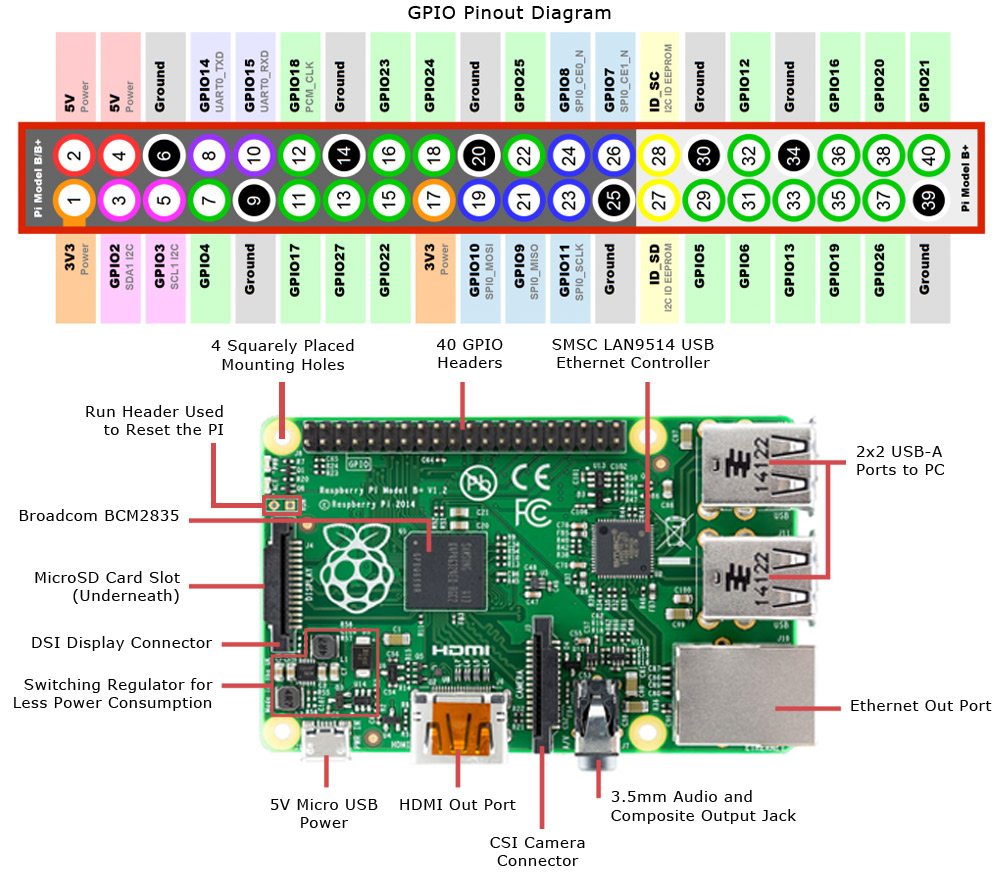
\includegraphics[width=0.8\textwidth]{../images/rpi2.jpg}	
			\caption{Popis \texttt{Raspberry Pi 2} a \texttt{GPIO}}
    		\label{fig:rpi2}
		\end{figure}
	
	
	
	
		\subsection{GPIO}
			\texttt{GPIO (General Purpose Input/Output)} je \texttt{40 pinů} umístěných na desce ve 2 řadách. Jednotlivé piny lze za běhu programově ovládat, všechny piny nejsou stejné, dělí se na několik skupin \texttt{napájení 5V}, \texttt{napájení 3v3}, \texttt{zem} a ostatní piny se od sebe ještě trošku liší, ale jedno mají společné, lze nastavit na \texttt{vstup/výstup}.
		
		
		\subsection{Operační systémy}
			\subsubsection{Raspbian}
				Raspbian je oficiální systém
			vychází z linuxové distribuce Debian
			Java, C++, Python, Nodejs
			\subsubsection{Windows 10 IoT Core}
				Sytém od Microsoftu Windows 10 IoT Core je systémem pro malé počítače a řídící elektroniku 
			c\#, C++, Python, Nodejs
			teprve v zacatcich
			webové rozhraní pro spravu
			potřeba visual studio k náhrání applikace
			
			knihovny pro GPIO v Alfa verzi
			
	\section{Čtečka RFID}
		\texttt{RFID (Radio-frequency identification)} používá elektromagnetické pole k automatické identifikaci. Byl navržen k identifikaci zboží jako náhrada za systém čárových kódů.\\
	\texttt{Tagy} obsahují uložené \texttt{identifikační číslo (UID)}, některé mají prostor pro další informace, do kterého lze ukládat. Pasivní \texttt{tagy} sbírají energii z blízké \texttt{RFID} čtečky k nabití svého napájecího kondenzátoru a odešlou rádiový signál. Aktivní \texttt{tagy} mají vlastní zdroj energie jako je baterie.\\
	Pro tento projekt se požije čtečka \texttt{RFID-RC522}, k \texttt{RPi} je připojí pomocí 7 \texttt{pinu} do \texttt{GPIO} viz. \ref{fig:gpio_rfid}.


\begin{figure}[h]
		\centering
		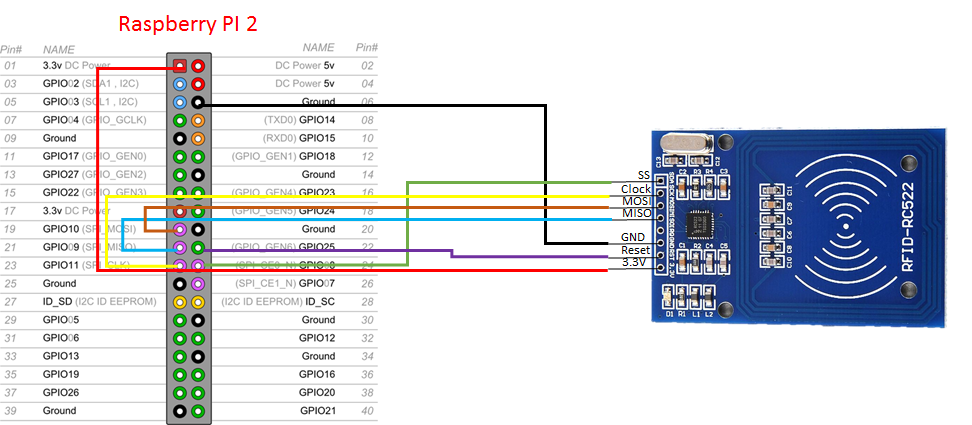
\includegraphics[width=0.8\textwidth]{../images/gpio_rfid.png}	
		\caption{Schéma zapojení \texttt{RFID-RC522} do \texttt{GPIO}}
		\label{fig:gpio_rfid}
	\end{figure}




\chapter{Analýzu problému}
	
		
	\section{Přidávání/odebírání zboží}
	\section{Informovat o stavu čtečky}
		k čemu je RFID, jak nám pomůžu
		Proveďte analýzu problému a zvolte vhodný programovací jazyk.
	
	\section{Návrh komunikace}
		\subsection{Komunikace s RFID čtečkou}
			MQTT
			diskutujte výhody/nevýhody vámi vybraného řešení
		
		\subsection{Komunikace s UI klientem}
			REST API
			diskutujte výhody/nevýhody vámi vybraného řešení
 
	\section{Zabezpečení}




				





\appendix
\bibliographystyle{csplainnat}
\bibliography{bakalarka}
\end{document}
